\documentclass[10pt]{beamer}
\usefonttheme{professionalfonts}
%\usetheme{CambridgeUS}
%
% Choose how your presentation looks.
%
% For more themes, color themes and font themes, see:
% http://deic.uab.es/~iblanes/beamer_gallery/index_by_theme.html
%
\mode<presentation>
{
  \usetheme{default}      % or try Darmstadt, Madrid, Warsaw, ...
  \usecolortheme{beaver} % or try albatross, beaver, crane, ...
  \usefonttheme{default}  % or try serif, structurebold, ...
  \setbeamertemplate{navigation symbols}{}
  \setbeamertemplate{caption}[numbered]
} 

\usepackage[english]{babel}
\usepackage[utf8x]{inputenc}
\usepackage{tikz}
\usepackage{pgfplots}
\usepackage{array}  % for table column M
\usepackage{makecell} % to break line within a cell
\usepackage{verbatim}
\usepackage{graphicx}
\usepackage{epstopdf}
\usepackage{amsfonts}
\usepackage{xcolor}
\usepackage{ifthen}
%\usepackage{mathtools}
\usepackage[makeroom]{cancel}
\usetikzlibrary{spy}
%\captionsetup{compatibility=false}
%\usepackage{dsfont}
\usepackage[absolute,overlay]{textpos}
\usetikzlibrary{calc, angles,quotes}
\usetikzlibrary{pgfplots.fillbetween, backgrounds}
\usetikzlibrary{positioning}
\usetikzlibrary{arrows}
\usetikzlibrary{pgfplots.groupplots}
\usetikzlibrary{arrows.meta}
\usetikzlibrary{plotmarks}
\usetikzlibrary{decorations.markings}
\usepgfplotslibrary{groupplots}
\pgfplotsset{compat=newest} 
%\pgfplotsset{plot coordinates/math parser=false}

\usepackage{hyperref}
\hypersetup{
    colorlinks=true,
    linkcolor=blue,
    filecolor=magenta,      
    urlcolor=cyan,
}

%
%\def\EXTERNALIZE{1}
%%% Page numbering
\usepackage{etoolbox} % necessary for excluding beamer-only frames from page numbering

\makeatletter
\pretocmd{\beamer@@@@frame}{\alt<#1>{}{\beamer@noframenumberingtrue}}{}{}
\makeatother

\addtobeamertemplate{navigation symbols}{}{%
	\usebeamerfont{footline}%
	\usebeamercolor[fg]{footline}%
	\hspace{1em}%
	\insertframenumber/\inserttotalframenumber
}
%%%

\definecolor{matlabcomment}{RGB}{34,139,34}

\pgfmathdeclarefunction{gauss}{1}{%
	\pgfmathparse{1/(sqrt(2*pi))*exp(-((#1)^2)/2)}%
}

\pgfmathdeclarefunction{laplacian}{2}{%
	\pgfmathparse{1/(#2*2)*exp(-(abs(x-#1))/(#2))}%
}

\pgfmathdeclarefunction{pretty_func}{1}{%
	\pgfmathparse{cos(deg(#1/2)) - sin(deg(#1)) + cos(deg(#1/2)-45) - sin(deg(#1/4)-154)}%
}

\pgfplotsset{
	dirac/.style={
		mark=triangle*,
		mark options={scale=2},
		ycomb,
		scatter,
		visualization depends on={y/abs(y)-1 \as \sign},
		scatter/@pre marker code/.code={\scope[rotate=90*\sign,yshift=-2pt]}
	}
}

\def\thickness{very thick}

\tikzset{
amark/.style 2 args={
	decoration={             
		markings, 
		mark=at position {0.5} with { 
			\arrow{stealth},
			\node[#2] {#1};
		}
	}, \thickness,
	postaction={decorate}
},
earlymark/.style 2 args={
	decoration={             
		markings, 
		mark=at position {0.25} with { 
			\arrow{stealth},
			\node[#2] {#1};
		}
	}, \thickness,
	postaction={decorate}
},
latemark/.style 2 args={
	decoration={             
		markings, 
		mark=at position {0.8} with { 
			\arrow{stealth},
			\node[#2] {#1};
		}
	}, \thickness,
	postaction={decorate}
},
zpath/.style={
	decoration={             
		markings, 
		mark=at position {0.5} with { 
			\arrow{stealth},
			\node[#1] {$z^{-1}$};
		}
	}, \thickness,
	postaction={decorate}
},
terminal/.style 2 args={draw,circle,inner sep=2pt,label={#1:#2}},
}


\tikzset{
	invisible/.style={opacity=0},
	visible on/.style={alt={#1{}{invisible}}},
	alt/.code args={<#1>#2#3}{%
		\alt<#1>{\pgfkeysalso{#2}}{\pgfkeysalso{#3}} % \pgfkeysalso doesn't change the path
	},
}

\newcommand\PlotSampledSpectrum[4]{%
	\def\fs{#2}%
	\def\fmax{#3}%
	\def\ros{#4}%
	\input{#1}%
}

\pgfmathdeclarefunction{invgauss}{2}{%
	\pgfmathparse{sqrt(-2*ln(#1))*cos(deg(2*pi*#2))}%
}

\tikzset{
	declare function={
		sinc(\x) = (and(\x!=0, 1) * (sin(deg(pi*\x))/(pi*\x)) +
		(and(\x==0, 1) * 1);
	}
}

\DeclareMathOperator{\E}{\mathbb{E}} % expectation

\newcolumntype{M}[1]{>{\centering\arraybackslash}m{#1}}

\definecolor{blue2}{RGB}{51, 105, 232}  
\definecolor{red2}{RGB}{213, 15, 37}  
\definecolor{green2}{RGB}{0, 153, 37}  
\definecolor{green3}{rgb}{0.1922, 0.6392, 0.3294}% 
\definecolor{yellow2}{RGB}{238, 178, 17} 
\definecolor{gray2}{RGB}{102, 102, 102}
\definecolor{orange2}{RGB}{230, 85, 13}

% Qualitative pallete set1 from www.ColorBrewer.org
\definecolor{Qred}{RGB}{228,26,28}
\definecolor{Qblue}{RGB}{55,126,184}
\definecolor{Qgreen}{RGB}{77,175,74}
\definecolor{Qpurple}{RGB}{152,78,163}
\definecolor{Qorange}{RGB}{255,127,0}
\definecolor{Qyellow}{RGB}{255,255,51}
\definecolor{Qbrown}{RGB}{166,86,40}
\definecolor{Qpink}{RGB}{247,129,191}
\definecolor{Qgray}{RGB}{153,153,153}

\newcommand\SimpleSys[4]{%
	\def\xin{#2}%
	\def\Hz{#3}%
	\def\yout{#4}
	\input{#1}%
} % some definitions

%% 
\title[EE 264]{Parametric Signal Modeling}
\author{Jose Krause Perin}
\institute{Stanford University}
\date{August 15, 2017}

\begin{document}

\begin{frame}
  \titlepage
\end{frame}

%
\begin{frame}{Last lecture}
	\begin{itemize}
	\item The PSD is the DTFT of the autocorrelation function
	\item The PSD may be two-sided or one-sided. Careful with conventions!
	\item The periodogram method estimates the PSD directly from the magnitude squared of the DFT of the windowed signal
	\item The periodogram is an biased estimator of the PSD, and it has large variance. Hence, the periodogram must be averaged to produce useful estimates
	\item The Welch method averages several periodograms
	\item The Welch method breaks the data into overalapping segments, each of length $L$. Usually, the segments overlap by $L/2$.
	\item Differently from the periodogram and Welch method, the Blackman-Tukey method estimates the PSD by computing the DFT of the estimated autocorrelation function
	\item Although the estimator of the autocorrelation function may be unbiased, the PSD estimate is biased. Windows with non-negative frequency response are typically preferred e.g., Bartlett
	\item Increasing the sequence length $Q$ improves accuracy. Reducing the window length $L$ improves accuracy at the expense of poorer frequency resolution.
\end{itemize}
\end{frame}

%
\begin{frame}{Parametric signal modeling}
	\begin{itemize}
		\item Another representation of signals
		\item We'll model \textit{complicated} signals as the output of some system to white noise or to an impulse.
		\item Hence, the signal will be described by the parameters (coefficients) of the system
		\item We'll cover the \textbf{all-pole model} or \textbf{autoregressive (AR) model}
	\end{itemize}
\end{frame}

\begin{frame}{All-pole model}
	\begin{center}
	\resizebox{0.5\linewidth}{!}{\begin{tikzpicture}[->, >=stealth, shorten >= 0pt, draw=black!50, node distance=3.2cm, font=\sffamily]
    \tikzstyle{node}=[circle,fill=black,minimum size=2pt,inner sep=0pt]
    \tikzstyle{block}=[draw=black,rectangle,fill=none,minimum size=1.5cm, inner sep=0pt]

	\node[node] (xc) {};
    \node[block, right=1cm of xc, text width = 1.5cm, align= center] (DSP) {$H(z)$};
	\node[node, right=1cm of DSP] (yc) {};
			
    \path (xc) edge (DSP);
    \path (DSP) edge (yc);
    
    \node[above = 0mm of xc, text width = 1cm, align=center] {$v[n]$};
    \node[above = 0mm of yc, text width = 3cm, align=center] {$\hat{s}[n] \approx s[n]$};
         
    \ifdefined\INVERSE
    	\node[block, right=1cm of yc, text width = 1.5cm, align= center] (inv) {$H^{-1}(z)$};
    	\node[node, right=1cm of inv] (xpred) {};
    	\node[above = 0mm of xpred, text width = 1cm, align=center] {$\tilde{v}[n]$};
	    \path (yc) edge (inv);
    	\path (inv) edge (xpred);
    \else\relax    	
    \fi
\end{tikzpicture}}
	\end{center}
	
	Given a signal $s[n]$, find $H(z)$ and $v[n]$ such that 
	\begin{equation*}
		s[n] \approx \hat{s}[n] = h[n] \ast v[n]
	\end{equation*}
	
	\begin{itemize}
		\item The \textbf{all-pole model} assumes
		\begin{equation*}
			H(z) = \frac{G}{1 - a_1z^{-1} - \ldots - a_{N}z^{-N}}
		\end{equation*}
		all zeros are at the origin
		\item If $s[n]$ is a \underline{finite-energy deterministic signal}, $v[n]$ is chosen to be an unit impulse
		\item If $s[n]$ is a \underline{WSS random process}, $v[n]$ is chosen to be a white noise process with unit average power
	\end{itemize}

	\textbf{Question:} how to find the coefficients $a_1, \ldots, a_N$?
\end{frame}


\begin{frame}{All-pole model}
Consider the inverse system
\begin{center}
	\def\INVERSE{1}
	\resizebox{0.9\linewidth}{!}{\begin{tikzpicture}[->, >=stealth, shorten >= 0pt, draw=black!50, node distance=3.2cm, font=\sffamily]
    \tikzstyle{node}=[circle,fill=black,minimum size=2pt,inner sep=0pt]
    \tikzstyle{block}=[draw=black,rectangle,fill=none,minimum size=1.5cm, inner sep=0pt]

	\node[node] (xc) {};
    \node[block, right=1cm of xc, text width = 1.5cm, align= center] (DSP) {$H(z)$};
	\node[node, right=1cm of DSP] (yc) {};
			
    \path (xc) edge (DSP);
    \path (DSP) edge (yc);
    
    \node[above = 0mm of xc, text width = 1cm, align=center] {$v[n]$};
    \node[above = 0mm of yc, text width = 3cm, align=center] {$\hat{s}[n] \approx s[n]$};
         
    \ifdefined\INVERSE
    	\node[block, right=1cm of yc, text width = 1.5cm, align= center] (inv) {$H^{-1}(z)$};
    	\node[node, right=1cm of inv] (xpred) {};
    	\node[above = 0mm of xpred, text width = 1cm, align=center] {$\tilde{v}[n]$};
	    \path (yc) edge (inv);
    	\path (inv) edge (xpred);
    \else\relax    	
    \fi
\end{tikzpicture}}
\end{center}

The inverse is an FIR system: $H^{-1}(z) = \frac{1}{G}(1 - a_1 - \ldots - a_Nz^{-N})$. Therefore,

\begin{equation*}
Gv[n] \approx s[n] - \sum_{k = 1}^N a_ks[n-k]
\end{equation*}

Defining the error
\begin{align*}
e_m[n] &= Gv[n] - \Big(s[n] - \sum_{k = 1}^N a_ks[n-k]\Big) \tag{modeling error} \\
\end{align*}

\end{frame}


\begin{frame}
We want to find coefficients $a_1, \ldots, a_n$ that minimize the \textbf{mean-square error}
\begin{equation*}
\langle |e_m[n]|^2 \rangle = \begin{cases}
\displaystyle\sum_{n =0}^{L} |e_m[n]|^2, & \text{$s[n]$ deterministic} \\
\E\Big(|e_m[n]|^2\Big), & \text{$s[n]$ random}
\end{cases}
\end{equation*}

From the properties of the mean-square error, it can be shown that the error is minimum when
\begin{equation*}
\langle s[n-i]e_m[n] \rangle = 0,  \quad i = 0, \ldots, N
\end{equation*}
The error is orthogonal to all inputs. This is known as the \textbf{orthogonality principle}
\end{frame}

%
\begin{frame}
Applying the orthogonality principle:

\begin{equation*}
\Big\langle s[n-i] \Big(Gv[n] - (s[n] - \sum_{k = 1}^N a_ks[n-k])\Big) \Big\rangle  = 0, \quad i = 0, \ldots, L
\end{equation*}

We'll only consider the cases when $i = 1, \ldots, N$:
\begin{align*}
	&\Big\langle s[n-i] \Big(Gv[n] - (s[n] - \sum_{k = 1}^N a_ks[n-k])\Big) \Big\rangle  = 0, \quad i = 1, \ldots, N \\
	&\langle s[n-i]s[n]\rangle - \sum_{k = 1}^N a_k\langle s[n-i]s[n-k]\rangle)  = 0, \quad i = 1, \ldots, N \tag{from causality $\langle s[n-i]v[n]\rangle = 0$}\\
\end{align*}

Note that $\langle s[l]s[m]\rangle$ is equivalent to either the \textbf{deterministic autocorrelation function} if $s[n]$ is deterministic, or $\langle s[l]s[m]\rangle$  is equivalent to the \textbf{autocorrelation function} if $s[n]$ is random
\begin{equation*}
	\langle s[l]s[m]\rangle = \begin{cases}
	c_{ss}[l-m], & \text{$s[n]$ deterministic} \\
	\phi_{ss}[l-m], & \text{$s[n]$ random}
	\end{cases}
\end{equation*}

\end{frame}

\begin{frame}
	If $s[n]$ is deterministic:
	\begin{equation*}
		c_{ss}[i] = \sum_{k = 1}^N a_kc_{ss}[k-i],  \quad i = 1, \ldots,N
	\end{equation*}
	
	
	If $s[n]$ is random: 
	\begin{equation*}
	\phi_{ss}[i] = \sum_{k = 1}^N a_k\phi_{ss}[k-i], \quad i = 1, \ldots,N
	\end{equation*}
	
	These equations are known as \textbf{normal equations} or \textbf{Yule-Walker equations}.
	
	\vspace{0.25cm}
	They form a system of $N$ linear equations of $N$ variables. Hence, there is at most one solution.
\end{frame}

\begin{frame}{In matrix notation}

Define
\begin{equation*}
	r[i] = \begin{cases}
	c_{ss}[i], & \text{$s[n]$ deterministic} \\
	\phi_{ss}[i], & \text{$s[n]$ random} \\
	\end{cases}
\end{equation*}
We can write the \textbf{normal equations} in matrix notation:
\begin{align*}
	Ra &= r \\
	\begin{bmatrix}
	r[0] & r[1] & \ldots & r[N-1] \\
	r[1] & r[0] & \ldots & r[N-2] \\
	\vdots & \vdots & \ddots & \vdots \\
	r[N-1] & r[N-2] & \ldots & r[0] \\
	\end{bmatrix}&\begin{bmatrix}
	a_1 \\
	a_2 \\
	\vdots \\
	a_N
	\end{bmatrix} = \begin{bmatrix}
	r[1] \\
	r[2] \\
	\vdots \\
	r[N]
	\end{bmatrix}
\end{align*}
$R$ is the \textbf{autocorrelation matrix}. Note that $R$ is symmetric $R = R^T$.

\vspace{0.5cm}
In Matlab: \texttt{>> a = R\textbackslash r}
\end{frame}

\begin{frame}{Determining the gain}
	Once the coefficients $a_1, \ldots, a_N$ have been found, we just need to determine the gain $G$ to completely specify $H(z)$.
	
	\vspace{0.5cm}
	We can pick $G$ so that the mean-square value of the model output matches the mean-square value of the signal $s[n]$:
	
	\begin{align*}
		\langle \hat{s}^2[n] \rangle &= \langle s^2[n] \rangle \\
		G^2 &= r_{ss}[0] - \sum_{k =1}^N a_kr_{ss}[k] \tag{after some algebra}
	\end{align*}
\end{frame}

\begin{frame}{Spectrum analysis with all-pole model}
	
	\textbf{Deterministic case:}
	\begin{equation*}
		|S(e^{j\omega})|^2 \approx |H(e^{j\omega})|^2|V(e^{j\omega})|^2 = |H(e^{j\omega})|^2
	\end{equation*}
	since by assumption $v[n] = \delta[n]$, it follows that $|V(e^{j\omega})|^2 = 1$
	
	\vspace{0.5cm}
	\textbf{Random case:}
	\begin{equation*}
	P_{ss}(e^{j\omega}) \approx |H(e^{j\omega})|^2P_{vv}(e^{j\omega}) = |H(e^{j\omega})|^2
	\end{equation*}
	since by assumption $v[n]$ is white noise, it follows that $P_{vv}(e^{j\omega}) = 1$
		
	\vspace{0.5cm}
	\textbf{Conclusion:}
	\begin{equation*}
		|H(e^{j\omega})|^2 = \bigg|\frac{G}{1 - \sum_{k =1}^Na_ke^{-j\omega k}}\bigg|^2
	\end{equation*}
	is the spectrum estimate of $s[n]$.
\end{frame}

\begin{frame}{All-pole analysis of speech signals}
	\centering
	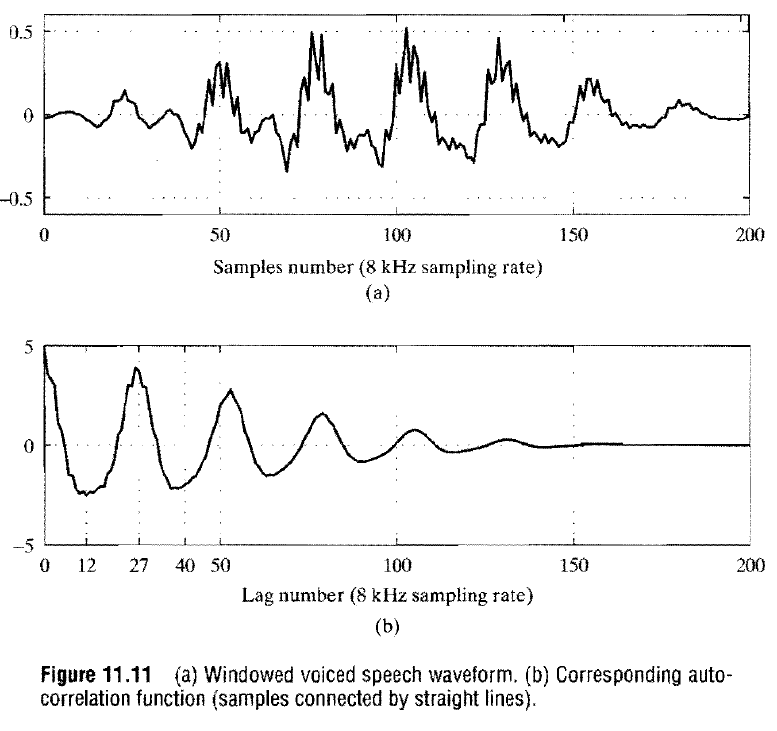
\includegraphics[scale=0.6]{figs/allpole_model_speech1.png}
\end{frame}


\begin{frame}{All-pole analysis of speech signals}
	\centering
	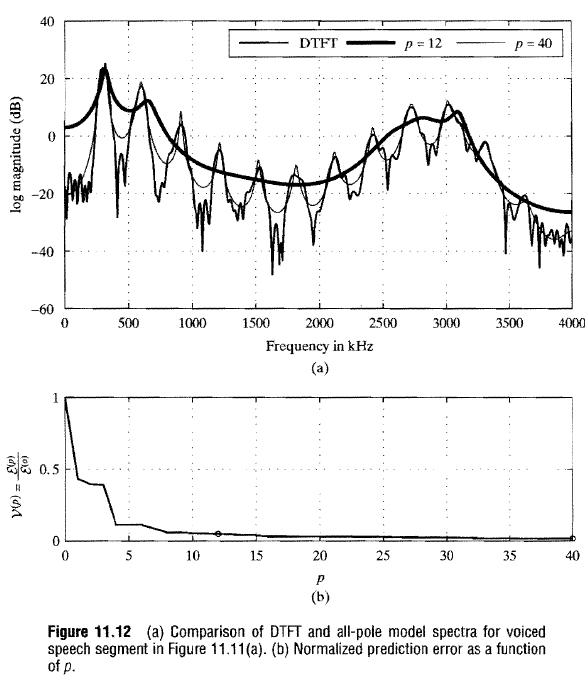
\includegraphics[scale=0.7]{figs/allpole_model_speech2.png}
\end{frame}

\begin{frame}{Revisiting the plant identification problem}
	
\begin{center}
	\resizebox{0.5\linewidth}{!}{\SimpleSys{figs/simple_in_dsp_out}{$x[n]$}{$H(z) = ??$}{$y[n]$}}
\end{center}

Inject a small noise of known PSD $\Phi_{xx}(e^{j\omega})$ at the input and measure the noise PSD at the output $\Phi_{yy}(e^{j\omega})$:

\begin{equation*}
|H(e^{j\omega})|^2 = \frac{\Phi_{yy}(e^{j\omega})}{\Phi_{xx}(e^{j\omega})} \tag{only know the magnitude}
\end{equation*}

We can obtain the phase response by computing the Hilbert transform of the log-magnitude
\begin{equation*}
\arg(H(e^{j\omega})) = -\mathcal{H}\{\ln |H(e^{j\omega})|\}
\end{equation*}

This procedure only works if $H(z)$ is causal and minimum phase i.e., it is stable and has a stable inverse.

\end{frame}

%
\begin{frame}{Summary}
	\begin{itemize}
		\item Parametric signal modeling is a form of representing complicated signals as the output to some system to an impulse or to a white noise process
		\item The all-pole or autoregressive model assumes that all zeros are at the origin
		\item Under the all-pole model the signal is described by the parameters $a_1, \ldots, a_N$, i.e., the system coefficients
		\item The coefficients can be determined by solving the normal equations, also known as Yule-Walker equations
		\item Solving these equations require estimates of either the deterministic autocorrelation function, if the signal is deterministic, or the autocorrelation function, if the system is random
		\item The magnitude square of the system is equivalent to the spectrum estimate of the signal
	\end{itemize}
\end{frame}

\end{document}
